\documentclass[11pt]{report}

\usepackage{epsf}
\usepackage{amsmath}
\usepackage{amsfonts}
\usepackage{subfigure}
\usepackage{placeins}
\usepackage{graphicx}
\usepackage{listings}
\usepackage{float}
\usepackage{algorithm}
\usepackage{algpseudocode}

\newcommand{\bdot}[0]{\boldsymbol{\cdot}}
\newcommand{\bunderline}[1]{\underline{\bf #1}}
\newcommand{\bvec}[1]{\vec{\bf #1}}
\newcommand{\sgn}[0]{\mbox{sgn}}
\newcommand{\pde}[2]{\frac{\partial {#1}}{\partial {#2}}}
\newcommand{\mDeriv}[1]{\frac{D {#1}}{D t}}
\newcommand{\deriv}[2]{\frac{d {#1}}{d {#2}}}
\newcommand{\subtext}[1]{{\mbox{\tiny #1}}}
\newcommand{\order}[1]{{O(#1)}}
\newcommand{\outprod}[0]{\otimes}
\newcommand{\half}[0]{\frac{1}{2}}
\newcommand{\third}[0]{\frac{1}{3}}
\newcommand{\fourth}[0]{\frac{1}{4}}
\newcommand{\D}[0]{\displaystyle}
\newcommand{\Dfrac}[2]{{\displaystyle \frac{#1}{#2}}}
\newcommand{\svec}[1]{{\Vec{#1}}}
\newcommand{\grad}[0]{\nabla}

\begin{document}

\title{Velocity Reconstruction, Interpolation \\ and Computing Back-Trajectories: \\
Requirements and Design}
\author{MPAS Development Team}

\maketitle
\tableofcontents

%-----------------------------------------------------------------------

\chapter{Summary}

The use of space-time transport algorithms, such Characteristic Discontinuous Galerkin (CDG) or Incremental Remapping (IR), requires the computation of Lagrangian pre-images. These pre-images are formed by tracing velocities defined at the vertices of the finite volume cells backward in time. In addition, some space-time algorithms such as CDG need to compute forward trajectories from arbitrary points within finite-volume cells.

The use of space-time transport algorithms requires the ability to 1) reconstruct full velocity vectors at vertices of finite-volume cells, 2) compute back-trajectories of these full velocity vectors and 3) the ability to determine the velocity vector at any point within a finite volume cell. MPAS-Ocean currently lacks the ability to do 1, 2 or 3. The code currently uses radial-basis functions to reconstruct velocity vectors at cell centers and this could readily be generalized to cell vertices.

This development contains three main challenges. First, we must construct full velocity vectors using nearby velocity component data. Second, we need to insure that back trajectories land in the ocean and not within land. And third, we need a sensible way to interpolate velocity vectors to any point within an ocean cell.

Ultimately we want this to work on the sphere, but this document is restricted to planar meshes as a starting point.

Success is as follows: Given the normal components of a linearly-varying velocity field at C-grid velocity points, the method exactly reconstructs this vector field at vertices and computes exact back trajectories. In addition, the vector velocity interpolation method at any point within the cell is exact for linearly-varying velocity vectors. This all points to a second-order accurate scheme. 

%figure template
%\begin{figure}
%  \center{\includegraphics[width=14cm]{./Figure1.pdf}}
%  \caption{A graphical representation of the discrete boundary.}
%  \label{Figure1}
%\end{figure} 




%-----------------------------------------------------------------------

\chapter{Requirements}

\section{Requirement: Vector Reconstruction at Vertices}
\label{Sec:Reconstruct}
Date last modified: 2012/11/01 \\
Contributors: (Todd Ringler) \\

The reconstruction of vector at vertices of finite volume cells (aka Voronoi cells) should be exact for linearly varying velocity fields. If we are given a velocity field

\begin{equation}
\label{eq:P}
{\bf P}({\bf x}) = (u({\bf x}),v({\bf x})) = (c_0 + c_1 x + c_2 y, d_0 + d_1 x + d_2 y)
\end{equation}
we compute the normal component of ${\bf P}$ at C-grid velocity points as

\begin{equation}
u_n({\bf x}_e) = {\bf P}({\bf x}_e) \cdot {\bf n}({\bf x}_e)
\end{equation}
where ${\bf x_e}$ are the location of C-grid velocity points and ${\bf n}_e$ are unit vectors normal to cell edges. Now using as much or as little $u_n({\bf x}_e)$ data as we choose, we compute

\begin{equation}
{\bf R}({\bf x}_v) = f(u_n({\bf x}_e))
\end{equation}
where ${\bf R}({\bf x}_v)$ the reconstruct vector velocity field at vertices based on $f$, the yet-to-be-determined reconstruction function. The requirement is that

\begin{equation}
{\bf R}({\bf x}_v) = {\bf P}({\bf x}_v)
\end{equation}
given (\ref{eq:P}). The above is just a fancy way of saying that we can exactly reconstruct linearly-varying velocity fields.


\section{Requirement: Vector Interpolation}
\label{Sec:Interpolate}
Date last modified: 2012/11/01 \\
Contributors: (Todd Ringler) \\

The vector interpolation of vector velocity at an arbitrary point within a Voronoi cells should be exact for a linearly-varying velocity field. Assuming that Requirement \ref{Sec:Reconstruct} is met, then we know the reconstructed velocity at cell vertices, ${\bf R}({\bf x}_v)$, is exact for linearly-varying functions. For an interpolated velocity, ${\bf I}$, evaluated at an arbitrary point, ${\bf x}_i$ within a cell, the requirement for interpolation is

\begin{equation}
{\bf I}({\bf x}_i) = {\bf P}({\bf x}_i)
\end{equation}
when the velocity has the form given in (\ref{eq:P}). The interpolated velocity can be constructed based on ${\bf R}({\bf x}_e)$ or $u_n({\bf x}_e)$ or both.

\section{Requirement: Back Trajectory Calculation}
\label{Sec:BackTrajectories}
Date last modified: 2012/11/01 \\
Contributors: (Todd Ringler) \\

Given ${\bf R}({\bf x}_v,t^n,t^{n+1})$ and a time step, $dt=t^{n+1}-t^n$, the method is required to find the point ${\bf x}_D(t^n)$

\begin{equation}
\label{eq:backtrajectory}
{\bf x}_D(t^n) = {\bf x}_v - \int_{t^{t+1}}^{t^n} {\bf I}({\bf x}_i,t^n,t^{n+1}) dt
\end{equation}
where ${\bf x}_i$ is along the back-trajectory characteristic and ${\bf x}_v$ is the location of a Voronoi vertex.

\subsection{Accuracy}
The accuracy requirement is that ${\bf x}_D(t^n)$ is exact for linearly-varying vector velocity fields. The notion of linearly-varying is extended here to include the time dimension.

\subsection{Bounds}
The bounds requirement is that ${\bf x}_D(t^n)$ is guaranteed to reside within the ocean domain.



%-----------------------------------------------------------------------

\chapter{Algorithmic Formulations}

\section{Design Solution: Vector Reconstruction at Vertices}
Date last modified: 2011/01/05 \\
Contributors: Todd Ringler and Pedro de Silva Peixoto \\

The vector reconstruction at cell vertices will be conducted using a least-squares solution using nearby normal-component velocity data points (reference Vidovic). Figure \ref{fig:least_squares} shows a portion of a Voronoi mesh. The solid circle at the vertex (call it $V$) is the location at which we wish to do a reconstruction. The algorithm will use the velocity component data along the edges connected to $V$ and the data along the edges connected to those edges. This results in 9 data values (nData=9) to be used in the reconstruction. Near boundaries, the recovery of 9 data values in a symmetric fashion is not possible. In those cases, we simply use the 9 closest velocity points. Each of these velocity data points are associated with a normal vector (shown in red in Figure \ref{fig:least_squares} to be referred to as ${\bf n}_k(x_k,y_k)$, where $k$ ranges from 1 to nData.

\begin{figure}
  \center{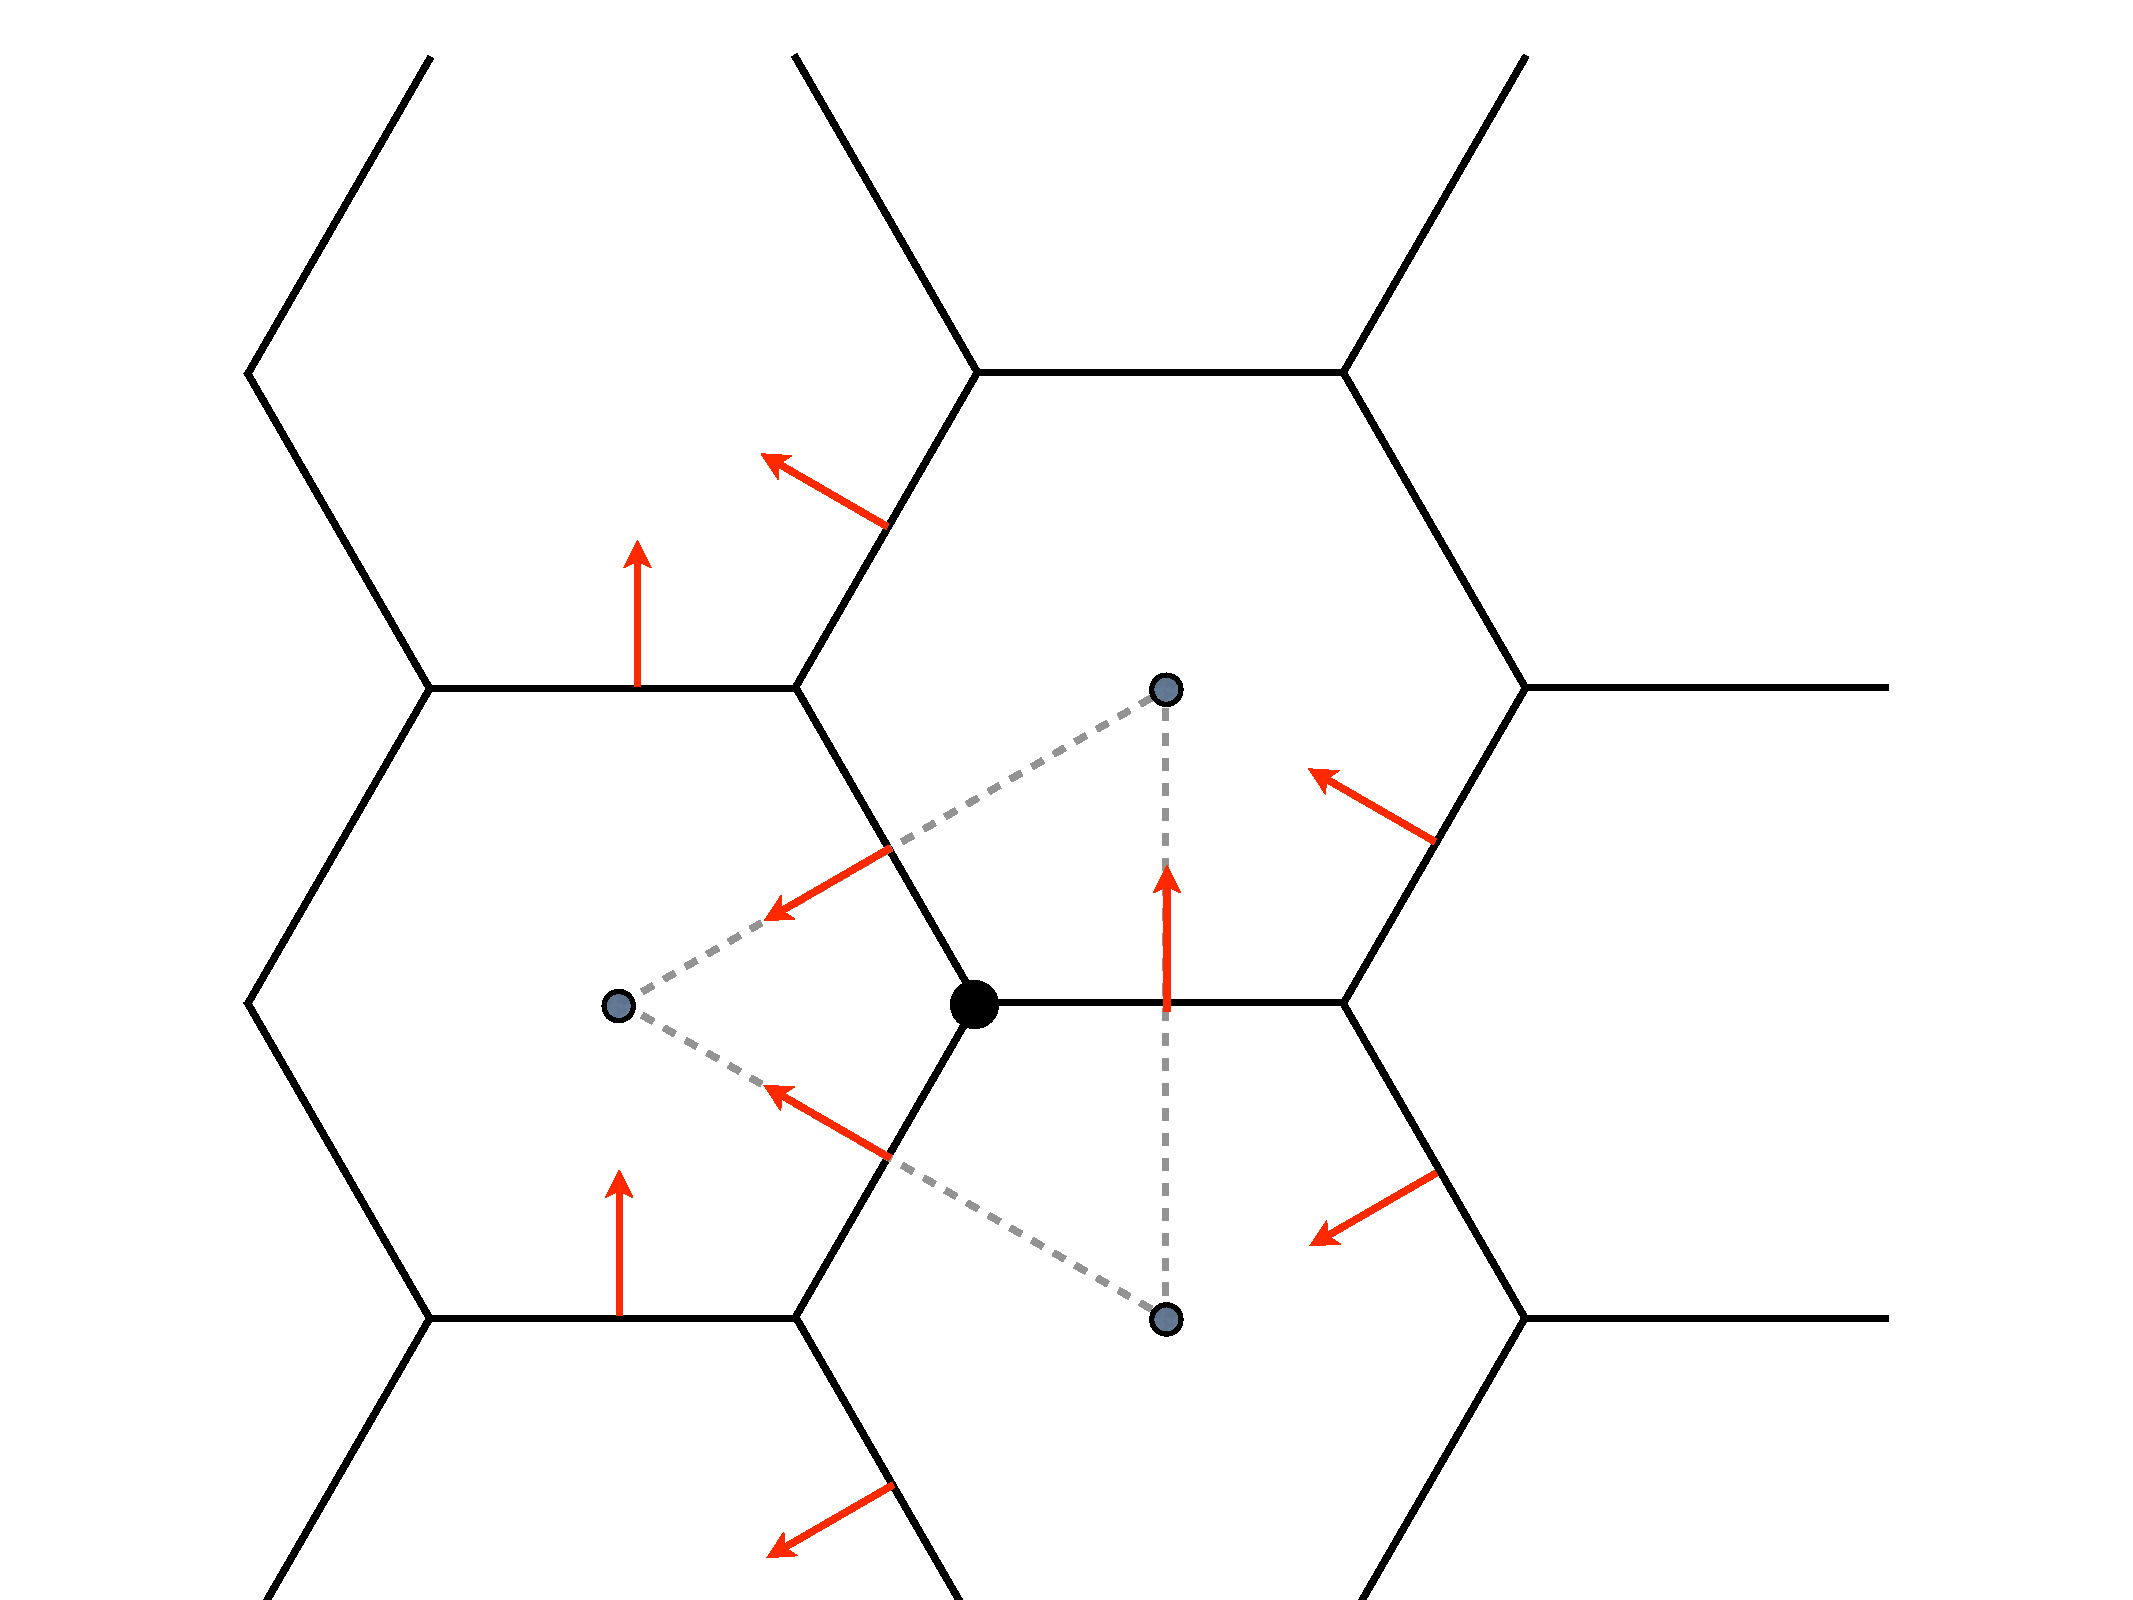
\includegraphics[width=14cm]{./least_squares.pdf}}
  \caption{Data used in least-squares reconstruction.}
  \label{fig:least_squares}
\end{figure} 

\begin{equation}
\begin{pmatrix} n_{x,1} & n_{x,1} x_1 & n_{x,1} y_1 &  n_{y,1} & n_{y,1} x_1 & n_{y,1} y_1  \\ 
                          \vdots & \vdots & \vdots & \vdots & \vdots & \vdots \\
                          n_{x,k} &  n_{x,k} x_k & n_{x,k} y_k & n_{y,k} & n_{y,k} x_k & n_{y,k} y_k
\end{pmatrix}
\begin{pmatrix} c_0 \\ c_1 \\ c_2 \\  d_0 \\ d_1 \\ d_2  \end{pmatrix} 
= 
\begin{pmatrix} u_{n,1} \\ \vdots \\ u_{n,k} \end{pmatrix}
\end{equation}
where the RHS is the normal-component velocity data. If we call the LHS matrix to be ${\bf M}$, tnhe least-squares solution is of the form

\begin{equation}
\begin{pmatrix} c_0 \\ c_1 \\ c_2 \\  d_0 \\ d_1 \\ d_2  \end{pmatrix}  = \left[ \left( {\bf M}^T {\bf M}\right)^{-1} {\bf M}^T \right] \begin{pmatrix} u_{n,1} \\ \vdots \\ u_{n,k} \end{pmatrix}.
\end{equation}
The matrix $\left[ \left( {\bf M}^T {\bf M}\right)^{-1} {\bf M}^T \right]$ will be computed at start up and stored at each vertex. If we set up a local coordinate system at each vertex with $(0,0)$ residing at the ${\bf x}_v$, then the reconstructed velocity is simply

\begin{equation}
{\bf R}({\bf x}_v) = (c_0, d_0)
\end{equation}
MATLAB code to test this least-squares reconstruction is here: \\
https://www.dropbox.com/s/69ql731ke1x8mwy/leastSquaresReconstruction.zip

\section{Design Solution: Vector Interpolation}
Date last modified: 2011/01/05 \\
Contributors: Todd Ringler and Pedro de Silva Peixoto \\

The velocity vector within a cell will be expressed as a function of the vector velocities at the cell vertices, i.e.

\begin{equation}
{\bf I}({\bf x}_i) = \sum_{k=1}^{nVert} \lambda_k {\bf R}_k
\end{equation}
where ${\bf x}_i$ is a point within the Voronoi cell, ${\bf R}_k$ is the set of vector velocities residing at vertices and $\lambda_j$ is the interpolation weight.

The interpolation weights are derived using Wachspress coordinates (reference Wachspress 1975 and Gillette paper), also known as generalized barycentric coordinates.  As shown in Figure \ref{fig:vector_interpolation}, each vertex will be associated with an area $B_k = T({\bf x}_{k-1},{\bf x}_k,{\bf x}_{k+1})$ where $T$ is the area of a triangle based on the location of its vertices. Note that $B_k$ is not a function of the interpolation point ${\bf x}_i$. Given an interpolation point ${\bf x}_i$, we now define $nVert$ triangles as $A_k = T({\bf x}_{k},{\bf x}_{k+1},{\bf x}_{i})$. The Wachspress coordinate is then

\begin{equation}
w_k({\bf x}_i) = B_k \prod_{l \ne k, l \ne k-1} A_l({\bf x}_i)
\end{equation}
and the interpolation weight for each vertex is then

\begin{equation}
\lambda_k({\bf x}_i)= \frac{w_k({\bf x}_i)}{\sum_{l=1}^{nVert} w_l({\bf x}_i)}
\end{equation}
The $\lambda$ functions can be thought of as non-negative, basis functions for each vertex. An example of one of these basis function is shown in Figure \ref{fig:Basis}. These basis functions have some very desirable properties for our application. First, $\lambda_k({\bf x}_{v,j})=1$ for $k=j$ and zero otherwise. Along an edge connecting two vertices, say $k$ and $k+1$, the interpolation is a linear function of $\lambda_k$ and $\lambda_{k+1}$ only. This results in $\lambda_k=0$ along all edges not connected to ${\bf x}_{v,k}$. The interpolation is exact for linear functions (reference). And finally, if we impose no-slip boundary conditions as ${\bf R}_k=0$ at boundary vertices, this zero-velocity condition holds exactly along all boundary edges. (Note: A special fix will be needed for those parts of the ocean domain that are only one-edge). 

MATLAB code to test Wachspress coordinates is here: \\ https://www.dropbox.com/s/oggd4iyekeqg3ng/WachspressCoordinates.zip

\begin{figure}
  \center{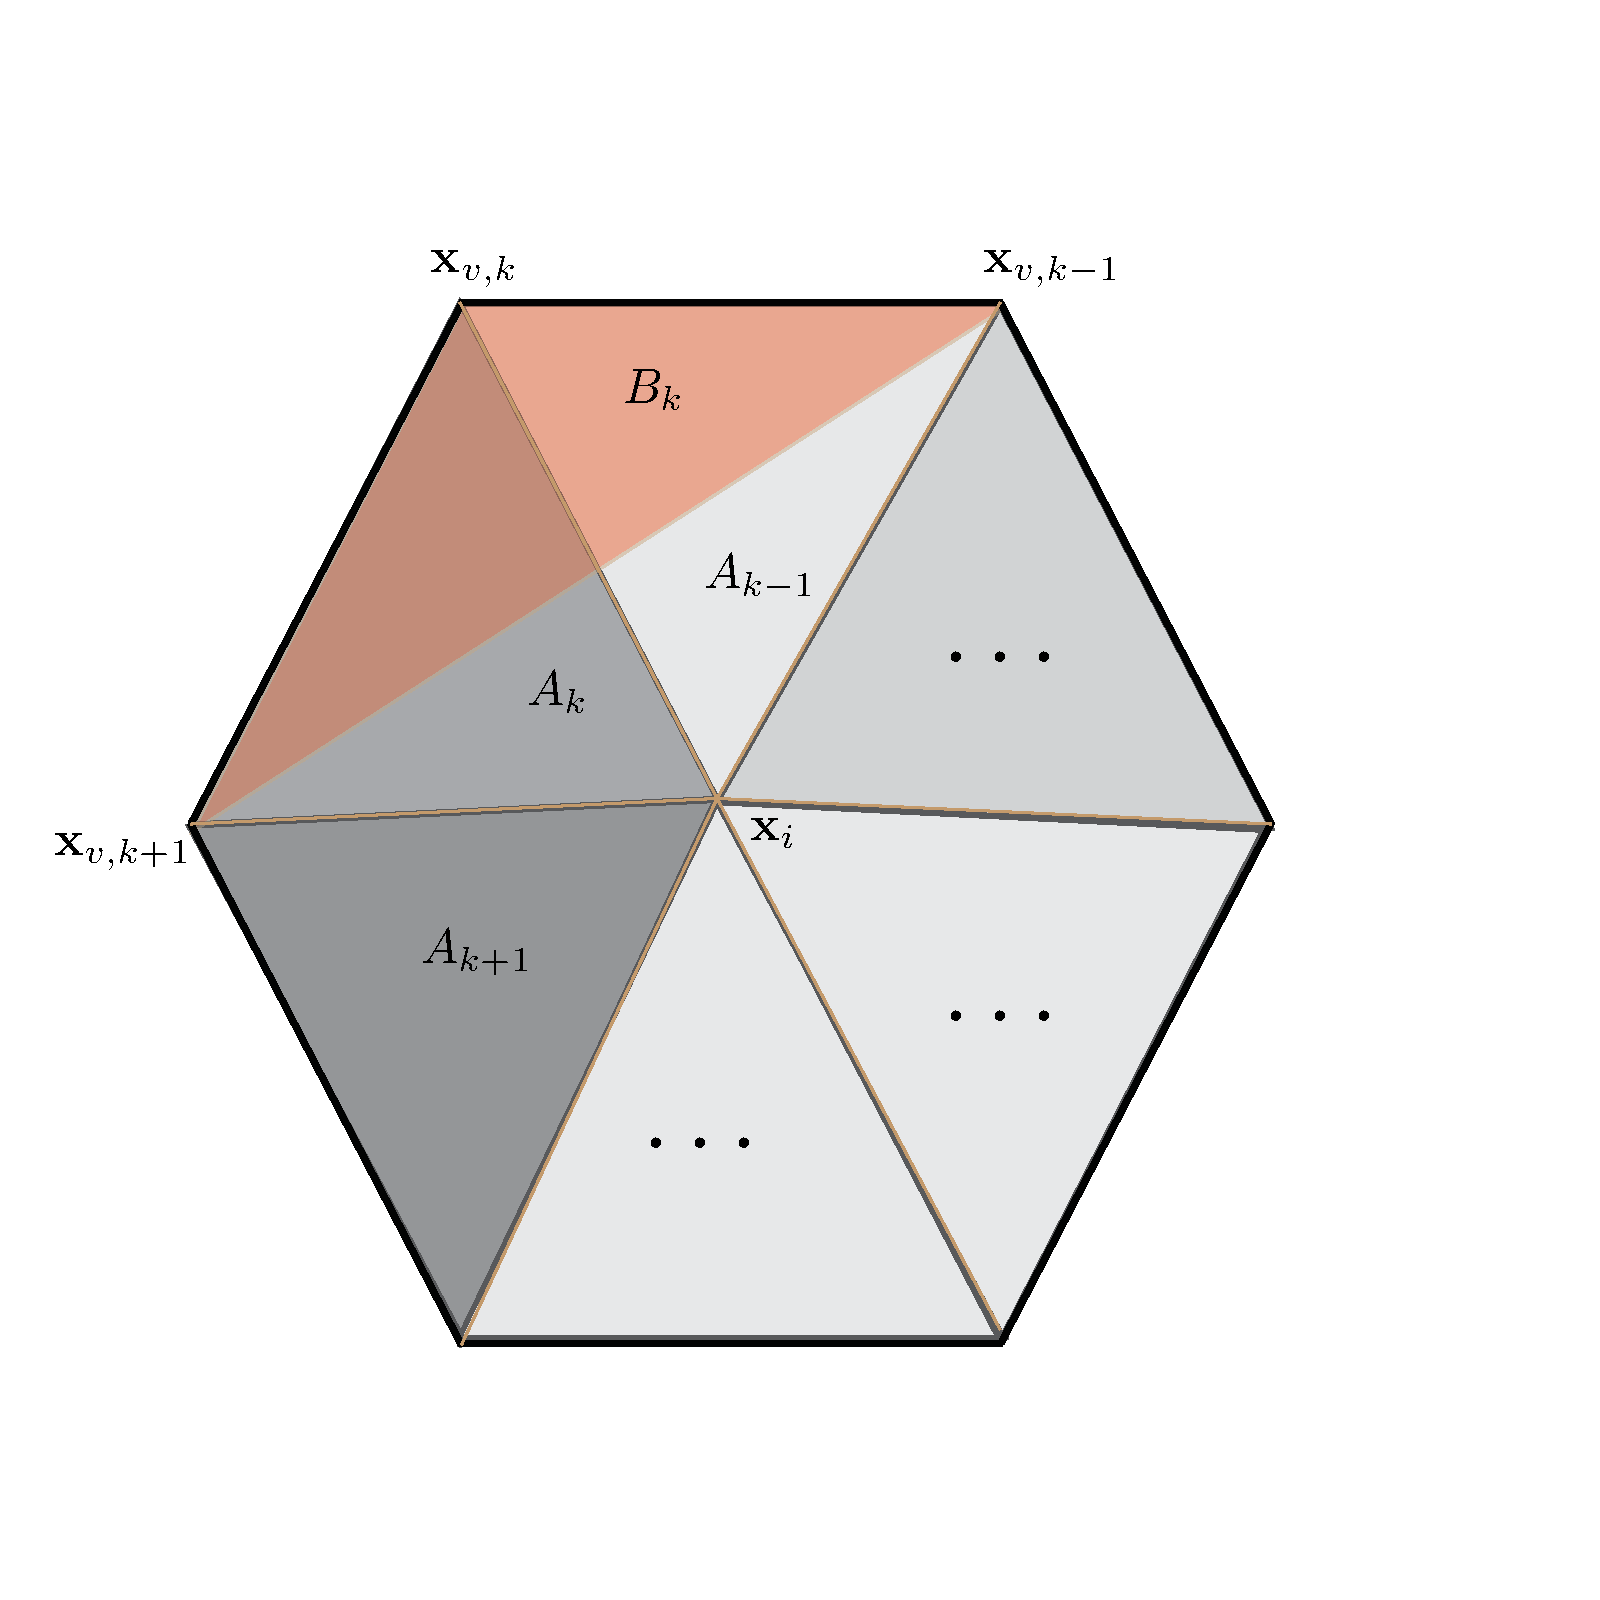
\includegraphics[width=14cm]{./vector_interpolation.pdf}}
  \caption{Interpolation of data to a point ${\bf x}_i$ based on vertex data defined at ${\bf x}_{v}$.}
  \label{fig:vector_interpolation}
\end{figure} 

\begin{figure}
  \center{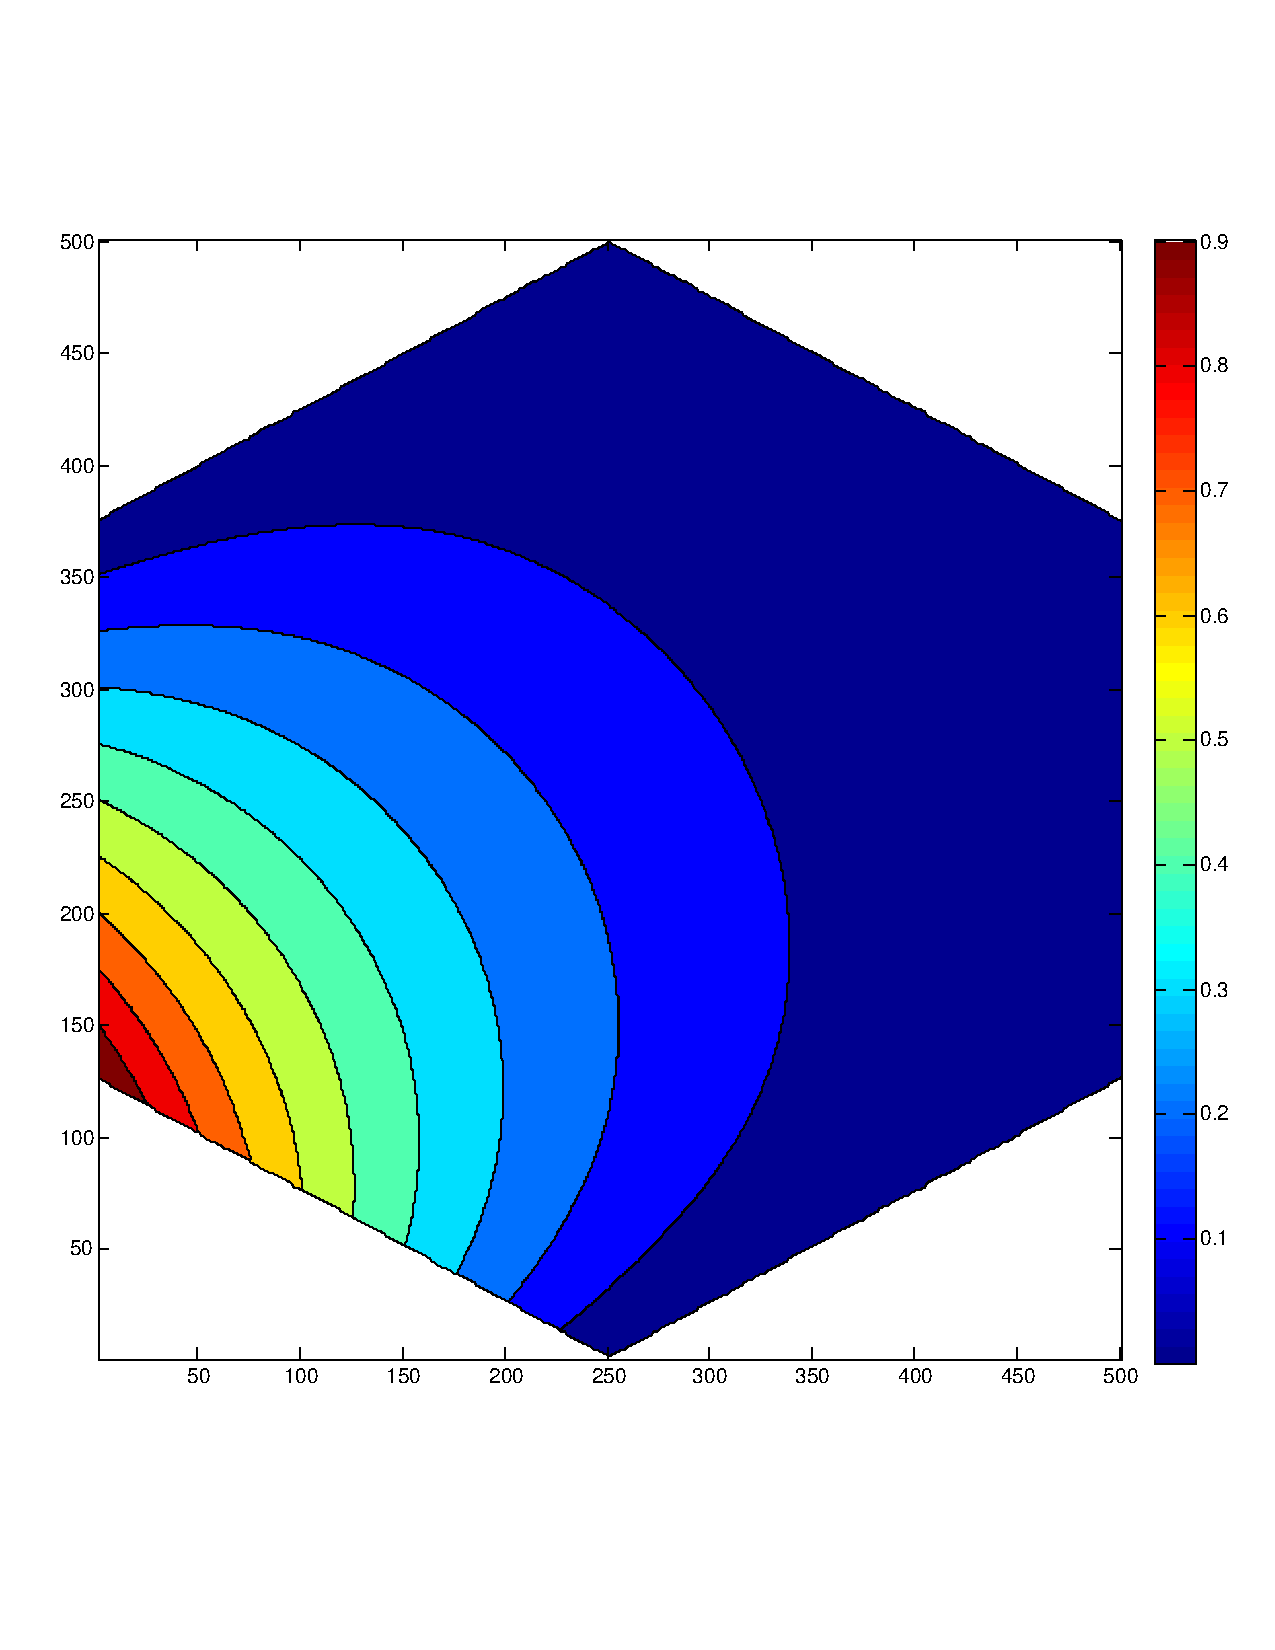
\includegraphics[width=12cm]{./gammaField.pdf}}
  \caption{Structure of a Wachspress basis function.}
  \label{fig:Basis}
\end{figure} 


\section{Design Solution: Backward Trajectories}
Date last modified: 2011/01/05 \\
Contributors: Todd Ringler and Rob Lowrie \\

The proposed algorithm is a self-correcting, mid-point rule for the integration along particle trajectories. The ``self-correcting''  nature of the algorithm is that if any points along the particle trajectory resides outside the ocean domain, the algorithm ``reboots'' automatically in order to do a more accurate trajectory calculation. By virtue of the mid-point (trapezoidal) integration, the scheme will be exact for linearly-varying flows in space and time. The algorithm outlined in Algorithm \ref{alg:back_trajectories} depends on the vector interpolation scheme described above in order to compute velocities at arbitrary locations within a Voronoi cell. Algorithm \ref{alg:back_trajectories} meets the accuracy and bounds requirements listed above.

\begin{algorithm}[ht]
  \caption{Calculation of backward particle trajectories}
  \label{alg:back_trajectories}
  \begin{algorithmic}[1]
    \State This algorithm is executed at every Voronoi vertex
    \State The algorithm should be valid for arbitrarily large CFL
    \State kLevel is the vertical layer in which to compute back trajectories
    \State $?_A$, $?_D$ and $?_{mid}$ are Arrival, Departure and mid-point {\it on each segment}
    \State nSegments is the number of line segments to be used in back trajectory
    \State nSegmentsMin will typically be 1
    \State nSegments=$\max$(nSegmentsLastTime-1,nSegmentsMin)-1
    \State kTest = -1 \Comment{Set to false so that do While loop is entered}
    \State ${\bf u}_A= {\bf u}_D={\bf u}^{n+1}_v$  \Comment{Initialize A and D velocities to be vertex velocity}
    \State ${\bf x}_D= {\bf x}_v$  \Comment{Initialize departure point to be vertex location}
    \For{While kTest $<$ 0} 
      \State kTest=1  \Comment{Assume it all works out}
      \State nSegments=nSegments+1
      \State dtSegment = dt / nSegments
      \For {iSegment=1,nSegments} \Comment{Integrate over segments}
      \State $t_D=t^{n+1}$-iSegment*dtSegment
      \State $t_A=t_D$+dtSegment
      \State ${\bf u}_A= {\bf u}_D$  \Comment{The arrival velocity is previous departure velocity}
      \State ${\bf x}_A= {\bf x}_D$  \Comment{The arrival point is previous departure point}
      \State ${\bf u}_{mid}= {\bf u}_D $ \Comment{Initialize midpoint velocity}
      \For {iter=1,nIterMidPoint} \Comment{Iterate to find midpoint values}
      \State ${\bf x}_{D}={\bf x}_A$-dtSegment*${\bf u}_{mid}$
      \State find iCellBase; ${\bf x}_{D}$ resides in iCellBase
      \State kTest = $\min$(maxLevelCell(iCellBase)-kLevel,kTest)
      \State Linearly interpolate ${\bf u}^n_v$ and ${\bf u}^{n+1}_v$ to ${\bf u}^n_v(t_D)$
      \State ${\bf u}_D$=vectorInterpolate(${\bf x}_{D},{\bf u}_v$(iCellBase,$t_D$))
      \State ${\bf x}_{mid}=1/2({\bf x}_{D}+{\bf x}_{A})$
      \State find iCellBase; ${\bf x}_{mid}$ resides in iCellBase
      \State kTest = $\min$(maxLevelCell(iCellBase)-kLevel,kTest)
      \State ${\bf u}_{mid}$=vectorInterpolate(${\bf x}_{mid},{\bf u}_v$(iCellBase,$t_{mid})$)
      \EndFor  \Comment{iter}
      \State ${\bf x}_{D} = {\bf x}_{A}$-dtSegment*${\bf u}_{mid}$
      \EndFor  \Comment{iSegment}
      \State if nSegments$>$nSegmentsMax then STOP
      \EndFor  \Comment{kTest}
      \State nSegmentsLastTime=nSegments
  \end{algorithmic}
\end{algorithm}


\section{Design Solution: Forward Trajectories}
Date last modified: 2011/01/05 \\
Contributors: Todd Ringler and Rob Lowrie \\
The proposed algorithm is identical to the backward trajectory Algorithm \ref{alg:back_trajectories} with two exceptions. First, the negative sign used in the backward trajectory to indicate backward-in-time is replace with a positive sign. This occurs on line 22 and 32. Second, the starting location and velocity is the set to the quadrature point and velocity at quadrature point instead of the vertex location and vertex velocity. Given the similarity between the forward and backward trajectory calculation, it is anticipated that both will be done with exactly the same source code.

%-----------------------------------------------------------------------

\chapter{Design and Implementation}

\section{Implementation: XXX}
Date last modified: 2011/01/05 \\
Contributors: (add your name to this list if it does not appear) \\

This section should detail the plan for implementing the design solution for requirement XXX. In general, this section is software-centric with a focus on software implementation. Pseudo code is appropriate in this section. Links to actual source code are appropriate. Project management items, such as svn branches, timelines and staffing are also appropriate.

How do we typeset pseudo code? 
\begin{verbatim}
  verbatim?
\end{verbatim}

%-----------------------------------------------------------------------

\chapter{Testing}

\section{Testing and Validation: XXX}
Date last modified: 2011/01/05 \\
Contributors: (add your name to this list if it does not appear) \\

How will XXX be tested? i.e. how will be we know when we have met requirement XXX. Will these unit tests be included in the ongoing going forward?


%-----------------------------------------------------------------------

\end{document}
